
\documentclass[a4paper,12pt,oneside]{article}
\usepackage[left=2.7cm,right=2.7cm,top=2.7cm,bottom=2.7cm]{geometry}


\usepackage{graphicx}
\usepackage{verbatim}
\usepackage{latexsym}
\usepackage{setspace}
\usepackage{titlesec}
\usepackage{tocloft}
\usepackage{hyperref}
\usepackage{color}
\usepackage{enumitem,kantlipsum}
\usepackage[authoryear]{natbib}
\bibliographystyle{typesetting/agsm1}
\usepackage{soul}
\usepackage{amsmath}

\hypersetup{hidelinks=true}
\usepackage{fontspec}
\setmainfont{LiberationSerif}
\setsansfont{LiberationSans}

%\renewcommand{\cftdot}{}
%\renewcommand{\cftsecleader}{\cftdotfill{\cftdotsep}}

\renewcommand\contentsname{}

\renewcommand\cftsecfont{\mdseries}
\renewcommand\cftsecpagefont{\mdseries}


\pagestyle{empty}

\setlength{\parskip}{2ex plus 0.5ex minus 0.2ex}
\setlength{\parindent}{0pt}

\makeatletter  %to avoid error messages generated by "\@". Makes Latex treat "@" like a letter

\def\submitdate#1{\gdef\@submitdate{#1}}
\def\cid#1{\gdef\@cid{#1}}
\def\wc#1{\gdef\@wc{#1}}

\def\maketitle{
  \begin{titlepage}{
    \raggedright
	
\includegraphics[width=7cm]{figures/logo}
	\myRule[mygray]{\textwidth}{2.5pt}
    \vskip 2.5cm
    \centering
    \Huge \@title \par
  }
  \vskip 2.5cm
  \par
  {\LARGE \textbf{\@author} \vskip 1.5cm \@submitdate}
 
  \vspace*{1.5cm}
  \large \textbf{Word Count: } \@wc
 
  \vspace*{1.5cm}
  \myRule[mygray]{\textwidth}{2.5pt}
  \vskip 0.5cm
  A thesis submitted in part fulfilment of the requirements for the degree of 
  \linebreak
  Master of Research at Imperial College London
  \linebreak \linebreak
  Formatted in the Journal style of Ecology Letters
  \linebreak \linebreak
  Submitted for the MRes in Computational Methods in Ecology and Evolution
  \end{titlepage}
}

\def\titlepage{
  \newpage
  \centering
  \linespread{1}
  \normalsize
  \vbox to \vsize\bgroup\vbox to 9in\bgroup
}
\def\endtitlepage{
  \par
  \kern 0pt
  \egroup
  \vss
  \egroup
  \clearpage
}


\def\preface{
    \pagenumbering{roman}
    \pagestyle{plain}
    \doublespacing
}

\def\body{
	\clearpage
	%\onehalfspacing
	\doublespacing
	\section*{Table of Contents}
	\tableofcontents
	\addtocontents{toc}{~\hfill\textbf{Page}\par}
	\clearpage
	\pagenumbering{arabic}
	\pagestyle{plain}
}

\makeatother  %to avoid error messages generated by "\@". Makes Latex treat "@" like a letter



\newcommand{\myRule}[3][black]{\textcolor{#1}{\rule{#2}{#3}}}
\definecolor{mygray}{gray}{0.8}



\titleformat{\section}
{\normalfont\Large}{\thesection}{1em}{}[{\color{mygray}\titlerule[1.3pt]}]

\titleformat{\subsection}
{\normalfont\large}{\thesubsection}{1em}{}[]




\begin{document}

\title{Using \emph{n}-dimensional Hypervolumes to measure Ecosystem Stability}

\author{David Bridgwood}
\submitdate{August 2018}
\wc{3516}

\maketitle

\preface
\clearpage

\section*{Declaration of Authorship}

\subsection*{Data Used}

All data from this thesis was provided by projects based at SAFE \citep{Ewers2011}. Data on trees came from Terhi Riutta \citep{Riutta2018}, small-mammals from Philip Chapman \cite{Chapman2018} and beetles from Adam Sharp (\url{https://www.safeproject.net/datasets/view_dataset?id=123}).

\subsection*{Analysis}

All code and analysis was undertaken by myself with the use of Python and R \citep{RCoreTeam2017}. The R package 'hypervolumes' \citep{Blonder2017a} was utilised in the construction of hypervolumes. All code is available at \url{https://github.com/dbridg15/masters_project}.

\subsection*{Supervision}

Prof. Rob Ewers and Dr. David Orme provided regular input on my analysis, suggesting possible methods and extensions.
\clearpage


\section*{Acknowledgements}

 \vspace*{5mm}

I would like to thank the following people for their contribution to the thesis:

 \vspace*{5mm}

\begin{itemize}
 \item My Supervisor Rob Ewers, for his guidance throughout the project.
 \vspace*{5mm}
 \item David Orme, for his help in developing my analysis.
 \vspace*{5mm}
 \item Samraat Pawar and James Rosindell for useful discussions about the project over the months.
\end{itemize}


\body
\normalsize
\section{Abstract}

\begin{enumerate}[leftmargin=*, label=\textbf{\arabic*.}]
	\item Set the context and purpose for the work; \\ \\ \\ \\
	\item Indicate the approach and methods used; \\ \\ \\ \\
	\item Outline the main results; \\ \\ \\ \\
	\item Identify the conclusions, the wider implications and the relevance to management or policy. \\ \\ \\ \\
\end{enumerate}


\textbf{Keywords:} 
\\ ecosystem stability, \emph{n}-dimensional hypervolumes, land-use change, SAFE.
\clearpage

\section{Introduction}

Ecosystems worldwide are experiencing escalating pressures from human influenced environmental changes including land-use and climate change \citep{Hautier2015}. Conversion of natural landscapes to agriculture and urban environments has been driven by continued population growth and increased demand for resources \citep{Green2005, Foley2005} significantly impacting global biodiversity \citep{Pimm1995}. These changes are shifting ecosystem communities away from historically stable states \citep{Hautier2015} and reducing their resilience to future environmental perturbations \citep{Oliver2015}. These biodiversity losses lead to reduced ecosystem function and services on which we rely \citep{Diaz2006, MillenniumEcosystemAssessment2005}.The impacts of these environmental changes are hard to predict \citep{Carpenter2009}, though globally ecosystem services are deteriorating \citep{Mace2012}.

Land-use changes are particularly prevalent in the tropical forests of Southeast Asia, a global biodiversity hotspot \citep{DeBruyn2014},  where selective logging for timber and conversion to oil palm plantations has significantly changed the structure of the rainforests which support such high biodiversity \citep{Gibson2011}. This logging has left degraded forest, fragments of old growth and oil palm plantations, all of which support a much lower species diversity than the continuous forests they replace \citep{Fitzherbert2008, Haddad2015} . These practices have been essential for the economic development of the region \citep{Basiron2007} but their impact has been significant on ecosystem processes \citep{Koh2011, Schleuning2011, Ewers2015}.  With demand for palm oil continuing to grow it is essential we learn to better manage these landscapes to mitigate any further impact \citep{Turner2008}.

\hl{MAKE BETTER} Large scale and long-term ecological field experiments are needed to provide this understanding, the Stability of Altered Forest Ecosystems Project (SAFE) is such a project \citep{Ewers2011}. Located in the Sabah, Malaysia the experiment covers a gradient of levels of forest modification with a fractal sampling design covering forest fragments of different sizes. Covering forest which is in the process of conversion to oil palm plantations it provides the perfect opportunity to study the impacts of this land-use change.

\subsection{Ecosystem stability}

Ecosystem stability can have a multitude of meanings \citep{Pimm1984}. It can be measured as: resilience; the time for the ecosystem to return to its equilibrium after a perturbation; resistance, the amount an ecosystem in changed by a perturbation; persistence, the time it takes before an ecosystem responds to the perturbation and variance, the degree to which an ecosystem varies though time. It is also possible to think of stability in terms of the number of possible stable states of a community, with more potential stable states resulting in a less stable system, increasing the likelihood of sudden shifts between ecosystem states \citep{Scheffer2001}. On top of this stability can be measured at a range of levels of complexity (e.g. species richness or community structure) which further multiplies the possible meaning of ‘stability’ \citep{Pimm1984,Lehman2000}.  It is therefore essential for studies to be explicit in what they are measuring and at which level of complexity as it is likely any relationships will differ between them. Temporal stability \citep{Tilman1999} is a measure of stability based on variance, it is defined as the mean abundance (\mu) of the species divided by the standard deviation (\sigma) of the variation in abundance through time $ \text{S = \mu/\sigma} $. This can be modified to assess the stability of a whole community (equation \ref{equ:temporal_stability}) \citep{Lehman2000}. This equation takes into account the variance of the system as well as how each possible pair of species covary together. From this we can see that the stability of a community increases with higher abundance and reduced variance and covariance. This equation can also be used to look at stability through space in place of time.

\vspace{0.3cm}

\begin{equation} \label{equ:temporal_stability}
\text{S\textsubscript{T}} = \frac{\text{\mu\textsubscript{T}}}{\text{\sigma\textsubscript{T}}} = \frac{\text{\Sigma \, Abundance}}{\sqrt{\text{\Sigma \, Variance + \Sigma \, Covariance}}}
\end{equation}


\vspace{0.3cm}

The relationship between ecosystem stability and biodiversity has been argued over in ecology for decades. Initial thoughts from \cite{Elton1958} and \cite{MacArthur1955} suggested that increasing biodiversity and complexity within a system would directly lead to higher stability. This seems intuitive as with greater species richness there is redundancy for species to fill function when others are lost, known as the insurance hypothesis \citep{Yachi1999}. However further theoretical work contradicted these ideas \citep{May1973} finding that increased diversity and community interactions decreased the stability of a system. Empirical studies have found that there is a positive relationship between diversity and temporal stability \citep{Tilman1994, Tilman2006}, with a systematic review by \cite{Ives2007} showing that a positive relationship was found in 69\% of studies on the topic. A number of explanations as to why diversity may increase stability have been proposed \citep{McCann2000}. \cite{Doak1998} suggested the Averaging effect, showing that even excluding interactions increasing species numbers on average reduced the variation in biomass due to statistical averaging, while \cite{Tilman1998} countered this with the Negative-Covariance effect which suggests that where species have a negative covariance, perhaps due to interspecific competition, this would generally stabilise the community. Regardless, it is clear that there is no simple link between stability and diversity \citep{Goodman1975}.

\hl{PARAGRAPH ON WHY TAXA!?}

\subsection{The \emph{n}-dimensional hypervolume}

An \emph{n}-dimensional hypervolume defines a volume in higher dimensional space. They have been used throughout ecology to represent systems with many components, allowing for a holistic approaching to assessing these components in combination.  \cite{Hutchinson1957} introduced the concept, using them to evaluate species niches. In his description each axis represents some independent environmental variable, physical or biological, with the hypervolume delineating the euclidean space that represents the environmental conditions which would allow the species to perpetuate. Since then the concept has been extended to incorporate axis of different kinds (climate, morphological traits, functional traits, etc.) measured at varying levels (communities, populations, species) to delineate hypervolumes in \emph{n}-dimensional space. Allowing questions about community composition \citep{Barros2016}, niche shifts \citep{Tingley2014, Blonder2015, Jackson2000, Evans2009}, functional richness \citep{Lamanna2014} and clade diversification \citep{Sidlauskas2008} to be explored. Recent developments allowing hypervolumes to be better delineated, especially in higher dimensions \citep{Blonder2014, Blonder2017b, Junker2016} provide potential for hypervolumes to become a common tool within ecology.

 
\cite{Barros2016} demonstrated that it is possible to use this concept of \emph{n}-dimensional to study the stability of ecosystems. They suggest that by describing an ecosystem state using axis from a range of ecosystem components before, during and after perturbation, the impact of the perturbation on the ecosystem state can be assessed. Using measures of hypervolume overlap, volume change and centroid movement the magnitude of change can be quantified. They highlight that studies on the rate of return to pre-perturbation state or new stable state could also be investigated. As a proof of concept they simulated climate change on European alpine plant communities and constructed two sets of hypervolumes at each time-step, one `community hypervolume' constructed using abundanced of plant functional groups, after a PCA to reduce dimensionality and the other using specific traits as the axis. Using measures of hypervolume change they assessed how the simulated ecosystem responded to the perturbation of climate change.


\subsection{Aims}

In this study I will use \emph{n}-dimensional hypervolumes, constructed to represent the community composition of trees, mammals and beetles at forest plots of different quality and logging history from SAFE. Comparing hypervolumes with a measure of overlap I will test the hypothesis that:

\begin{itemize}
	\item ecosystems with greater biomass will be more stable \citep{Tilman2006}, with the expectation that plots with higher biomass will have higher levels of hypervolume overlap.
	\item longer lived taxa will have more stable communities with greater hypervolume overlap
\end{itemize}
 
 I will investigate how measures of stability using hypervolumes compare to the more established community-stability \citep{Lehman2000}.
 	

\section{Materials and Methods}


\subsection{Study Sites and Data Collection}

	Data for all taxa was taken from studies based at the SAFE project in Sabah, Malaysia \citep{Ewers2011} as summarised in Table S\ref{sup:table1}. This project covers forest across a gradient of disturbance levels and attempts to control for confounding variables (i.e. slope, elevation and latitude) in its experimental design. 

	\subsubsection*{Trees}
	
	All plots had a total area of 1 ha, split into 25 subplots each $\text{20m} \times \text{20m}$. Plots were censused at least twice with the majority having four censuses between 2011 and 2016. At each census all trees with stem diameter >10 cm at 1.3m height were identified to species level, diameter was measured and height estimated \citep{Riutta2018}. From these measurements aboveground biomass (AGB) of each tree was predicted from allometric equations for moist tropical forest \citep{Chave2005}. From this data I created a species by subplot-census matrix, where each subplot would act as a unique point in the construction of hypervolumes. The AGB from the data was used as the score for each plot, taking the median of subplots.

	\subsubsection*{Mammals}
	
	For a detailed description of small-mammal trapping at SAFE see \cite{Wearn2017} and \cite{Chapman2018}. In summary plots were split into 6 grids each with 48 trapping locations spaced 23m apart. In each census year each trapping location was sampled on 7 consecutive nights, with two traps set at each trap location. Mammals were identified to species level, tagged, aged and sexed. For the purpose of my analysis I summed each trap location for each year, creating a species by trap-year matrix, where each trap acts as a unique point in the construction of the hypervolumes. AGB measures exist at all 2\textsuperscript{nd} order sampling points of SAFE \citep{Pfeifer2016}, each mammal trap was assigned the value of the closest 2\textsuperscript{nd} order site with the AGB score of each plot calculated as the median for all traps.
	
	
	\subsubsection*{Beetles}
	
	Beetles were sampled at the 1\textsuperscript{st} fractal order sites of SAFE with a combination trap (pitfall, flight-interception, malaise) left for 3 days and identified to family level \hl{(citation would be great)}. Each trap location was censused in at least two discrete time-points and for this analysis each trap acts as a unique point in the construction of the hypervolumes. The AGB score for these was calculated by assigning each sampling site with its corresponding 2\textsuperscript{nd} order AGB measurement, then taking the median of all these traps.
		
\subsection{Dimension Reduction and Hypervolume Calculation}
	
	
    To reduce the data to an appropriate number of dimensions for hypervolume calculation and establish orthogonality, I carried out Principal Component Analysis (PCA). This was performed on the raw abundance data for each taxa separately but with all subplots and censuses included, allowing hypervolumes constructed from subsets of the output to be comparable. The PCA was performed using the 'rda' function from the R package vegan \citep{Oksanen2018}.	
	
	Before hypervolumes were calculated, points from the PCA output were adjusted so all census steps would be standardised to one-year. The trajectory of each point between censuses was determined and the points position at time = 1 year calculated and used to construct hypervolumes for census n + 1. Time between censuses was defined as the middle day of census two minus the middle day of census one.
	
	\subsubsection*{Construction of Hypervolumes}
	Hypervolumes were constructed using the R package 'hypervolumes' \citep{Blonder2017a}. This uses a Gaussian kernel density estimation to delineate n-dimensional hypervolumes. See \cite{Blonder2014, Blonder2017b} for a detailed description of the algorithms, but in brief
	\begin{enumerate*}[label=(\roman*)]
		\item random points are drawn from hyperellipses surrounding each observation
		\item a uniform density is formed by resampling these points
		\item kernel density estimate was calculated at each random point
		\item the hypervolume is then defined by those points above a threshold value.
	\end{enumerate*}  
		
	For trees, subplots acted as individual observations, while traps were used for mammals and beetles, from these observations seperate volumes were delineated for each plot and census, after time steps were standardised to one year. All hypervolumes were constructed using the first three principal components from the PCA, this was due to data constraints as increasing the number of dimensions quickly leads to disjunct hypervolumes, \cite{Blonder2017b} suggest the maximum number of dimensions should not exceed $\ln m$ where $m$ is the number of observations from which the hypervolume is constructed.

\subsection{Comparison of Hypervolumes and Effect of Above Ground Biomass}

Comparisons were carried out between census steps for hypervolumes of the same plots to assess the variation in community composition through time. A measure of overlap, the Jaccard Similarity (volume of intersection divided by volume of union) and the distance between hypervolume centroids was taken, both using functions from the hypervolumes package \citep{Blonder2017a}.

	The average overlap for each taxa was compared using an analysis of variance (ANOVA) to establish if any significant differences existed, with a post-hoc Tukey HSD to establish where any significance between taxa existed. 






\subsection{Spatial Stability}
Was calculated for each plot/census - same Jazz...
\\
\\
\\

\section{Results}

Across all the censuses and traps/subplots, the data contained 666 species of trees, 26 species of small-mammals and 58 families of beetles. Output from the PCAs performed on each taxa separately but including all subplots/traps and census indicated that the first 3 components explained 28.89\%, 5.65\%, 4.44\% (cumulative 38.98\%) for trees, 26.44\%, 24.03\%, 11.34\% (cumulative 61.81\%) for mammals and 88.33\%, 7.59\%, 1.87\% (cumulative 97.79\%) for beetles.


\subsection{Comparison of Hypervolumes}

Hypervolumes were constructed for all plots and census and each census step within plots was compared. Figure \ref{fig:1} shows an example of a stable plot with little change in hypervolume shape leading to high levels of overlap and a comparatively unstable plot where significant changes in shape and size of the hypervolume lead to smaller measure of overlap and greater distance between centroids.

\begin{figure}[H]
	\centering
	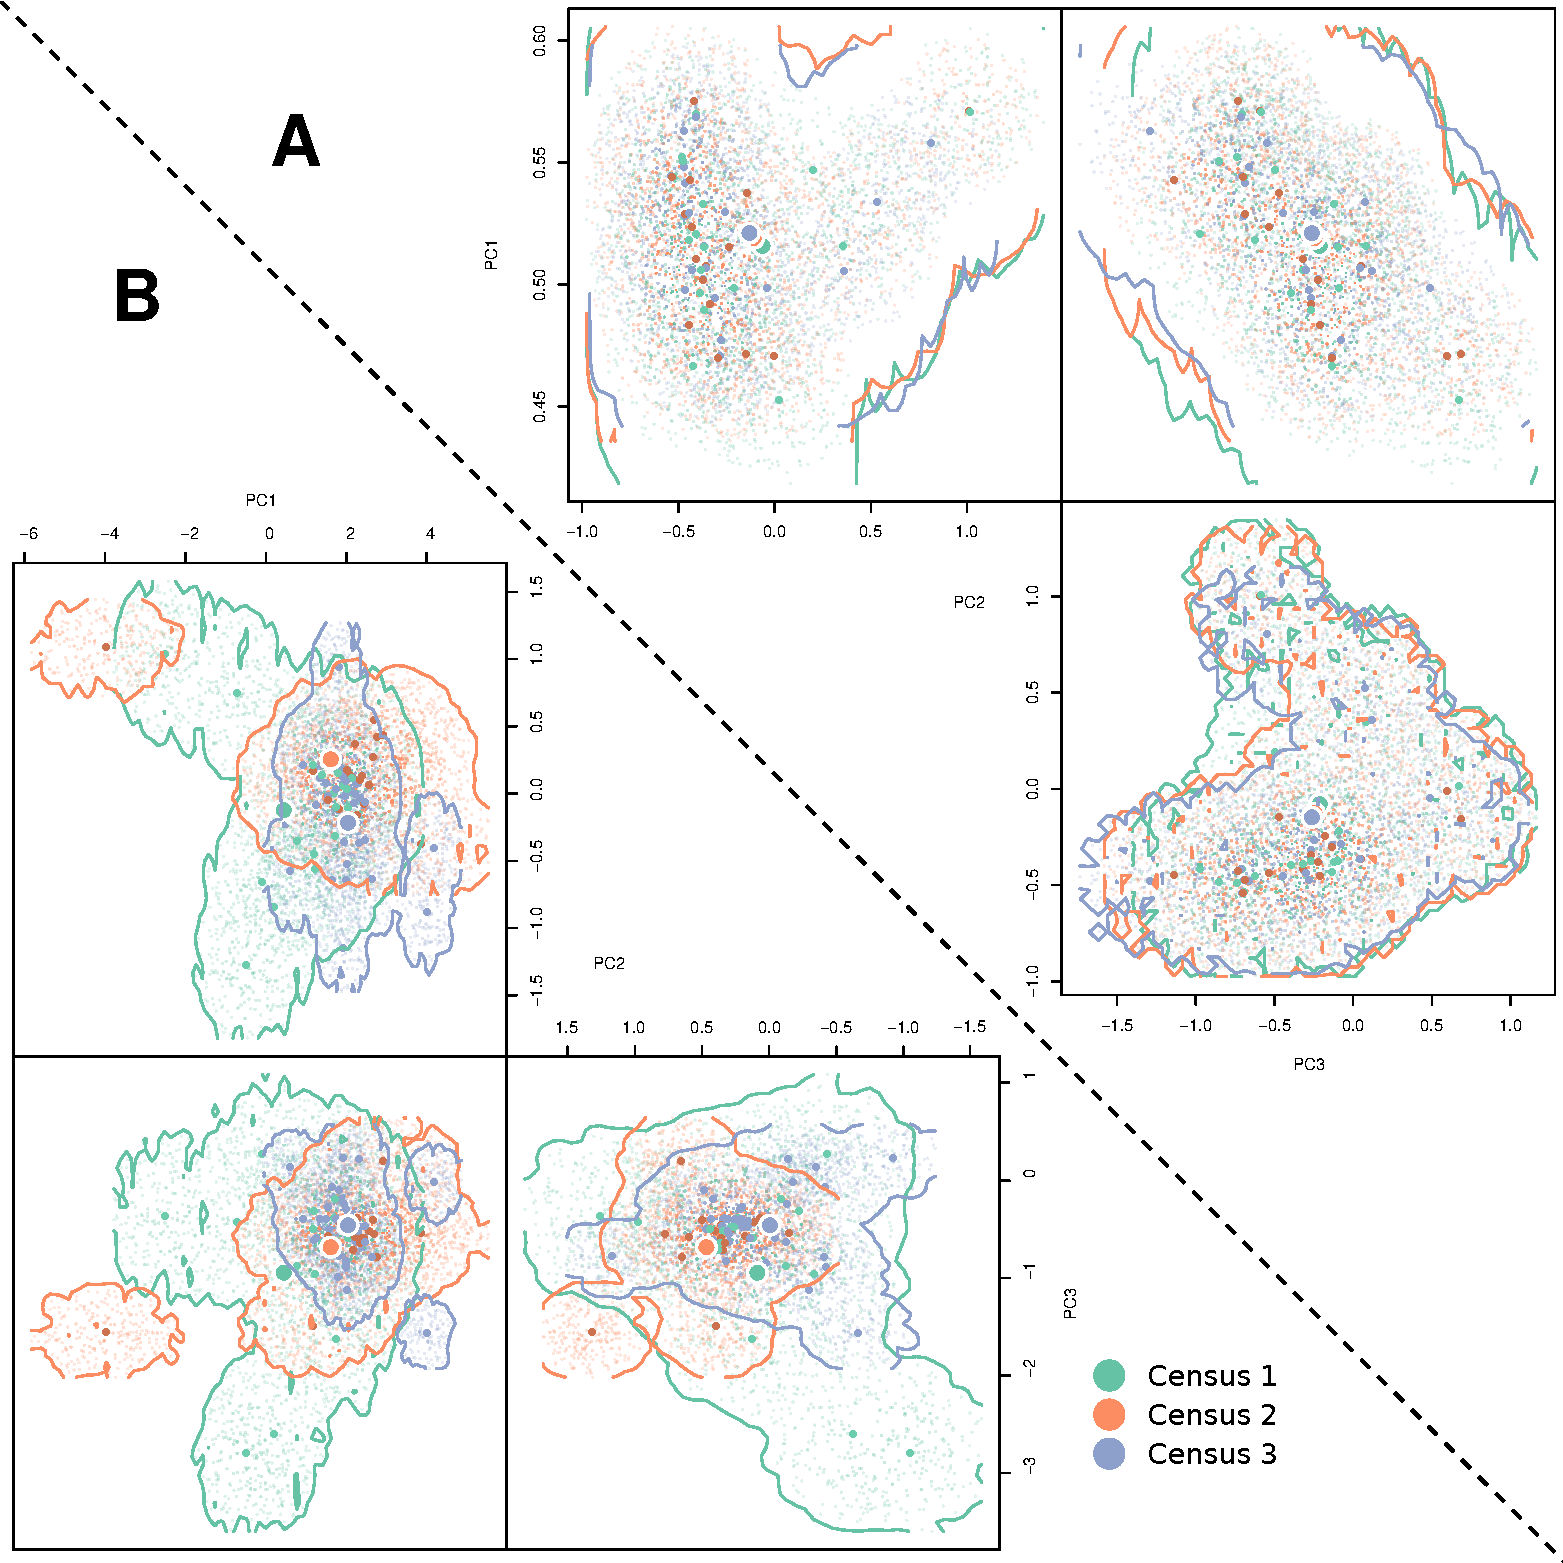
\includegraphics[width=\textwidth]{figures/figure1.pdf}
	\caption{(A) Hypervolumes constructed from tree community data at the Belian plot, an example of a plot with high levels of hypervolume overlap (mean = 0.802). (B) Hypervolume constructed from beetles community data at plot D, an example of comparativley low hypervolume overlap (mean = 0.243)}
	\label{fig:1}
\end{figure}	


\subsection{Effect of Taxa and Aboveground Biomass}

A one-way ANOVA found a significant difference in hypervolume overlap between taxa (F(2, 60) = 151.1, p < 0.001), with a post-hoc Tukey HSD finding that trees have significantly higher levels of overlap when compared with mammals or beetles (p < 0.001) (figure \ref{fig:2} A \& B), while no difference was found between the other taxa. No significant effect of AGB was found to exist with the level of hypervolume overlap in any of the taxa, results summarised in Table \ref{tab:hv-ovlp}.

\begin{figure}[H]
	\centering
	\includegraphics[width=\textwidth]{figures/figure2.pdf}
	\caption{(A) Difference in hypervolume overlap between taxa. (B) Effect of AGB on hypervolume overlap. (C) Difference in temporal community stability between taxa. (B) Effect of AGB on temporal community stability.}
	\label{fig:2}
\end{figure}

\begin{table}[H]
	\singlespacing
	\caption{Summary of results from ANCOVA assessing the relationship of taxa and AGB to hypervolume overlap}
	\label{tab:hv-ovlp}
	\begin{tabular*}{\textwidth}{c @{\extracolsep{\fill}} @{}llllll@{}}
		\toprule
		& \textbf{Df} & \textbf{Sum Squares} & \textbf{Mean Square} & \textbf{F Value} & \textbf{p} \\ \midrule
		log(AGB)    & 1  & 0.049       & 0.0492      & 3.043   & 0.087   \\
		Taxa        & 2  & 5.026       & 2.5128      & 155.439 & < 0.001 \\
		Interaction & 2  & 0.066       & 0.0332      & 2.053   & 0.138   \\
		Residuals   & 57 & 0.921       & 0.0162      &         &         \\ \bottomrule
	\end{tabular*}
\end{table}


\subsection{Community Temporal Stability}

A similar pattern was found with this more traditional measure of stability, with trees having significantly higher levels of temporal stability than either of the other taxa (F(2, 27) = 46.79, p < 0.001). With this measure there was an effect of AGB on the stability in trees (figure \ref{fig:2}D) however again this did not exist for the other taxa results summarised in Table \ref{tab:stb-ovlp}.

\begin{table}[H]
	\singlespacing
	\caption{Summary of results from ANCOVA assessing the relationship of taxa and AGB to community temporal stability}
	\label{tab:stb-ovlp}
	\begin{tabular*}{\textwidth}{c @{\extracolsep{\fill}} @{}llllll@{}}
		\toprule
		& \textbf{Df} & \textbf{Sum Squares} & \textbf{Mean Square} & \textbf{F Value} & \textbf{p} \\ \midrule
		log(AGB)    & 1  & 6.31       & 6.306      & 13.063   & 0.001   \\
		Taxa        & 2  & 57.09       & 28.545      & 59.133 & < 0.001 \\
		Interaction & 2  & 4.45       & 2.223      & 4.605   & 0.0203   \\
		Residuals   & 24 & 11.59       & 0.483      &         &         \\ \bottomrule
	\end{tabular*}
\end{table}

A significant Pearson's correlation was found between this new measure of stability 'Hypervolume Overlap' and the community temporal stability for each plot (r = 10.93, df = 28, p < 0.001) (figure \ref{fig:3}). However this relationship did not exist when looking at individual taxa in turn, with the exception of trees (r = 3.82, df = 7, p = 0.007).

\begin{figure}[H]	
	\centering
	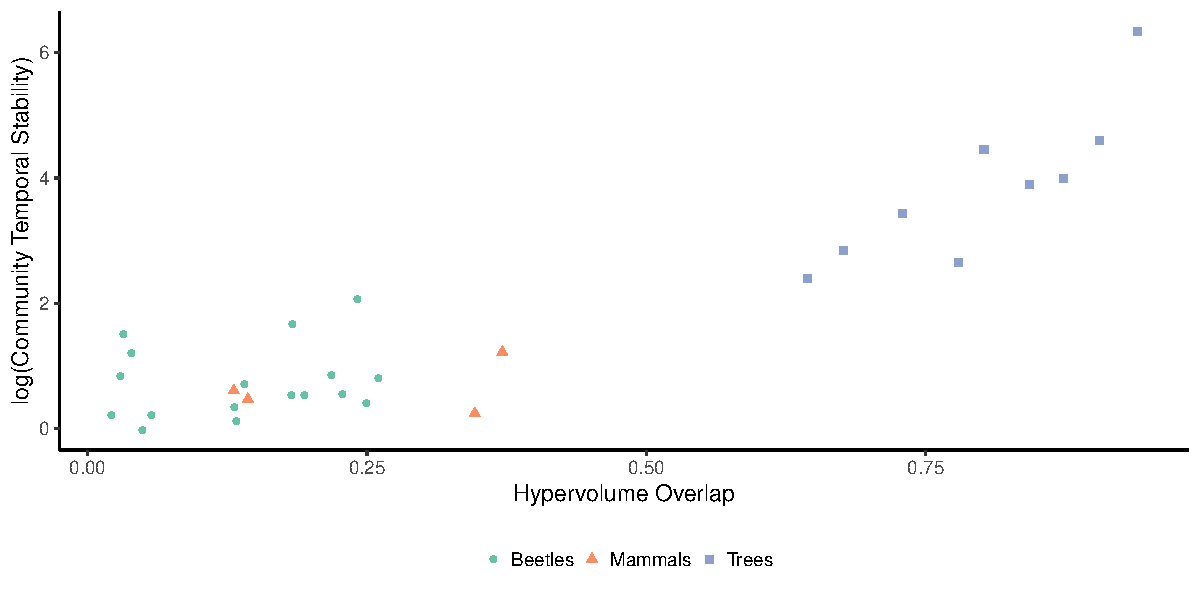
\includegraphics[width=\textwidth]{figures/figure3.pdf}
	\caption{The relationship between hypervolume overlap and temporal community stability. A significant Pearson's correlation was found overall (r = 10.93, df = 28, p < 0.001). However when split into separate taxa only trees had a significant correlation (r = 3.82, df = 7, p = 0.007)}
	\label{fig:3}
\end{figure}


\section{Discussion}

This project attempted to study ecosystem stability in a new way, using n-dimensional hypervolumes to represent the state of ecosystem communities and assess the variation in these hypervolumes between censuses at plots of varying forest quality.  

Hypervolume overlap between censuses was found to be significantly higher in tree communities than in either mammals or beetles, the other two taxa studied. This suggests that trees are overall more stable as a taxa. However, no significant relationship was found between the AGB (a continuous measure of forest quality) of the plot and the hypervolume overlap and so stability of communities within. This is contrary to what is predicted by theory \citep{MacArthur1955, Hughes2000a} and has previously been found by empirical studies \citep{Tilman2006, Ives2007}, where increased biomass has been associated with greater stability of ecosystems. These measures of stability using hypervolume overlap were also compared with the more traditional measure of community temporal stability \citep{Lehman2000} which produced similar results. Using this more traditional measure still found no relationship between AGB and stability. 

Trees were found to be significantly more stable, with greater levels of hypervolume overlap than either of the other taxa tested. Given that stability was measured at the scale of years this is not a surprising result as the generation length is higher and so turnover of trees is much lower than either of the other groups \citep{Connell1983, Pimm1984}. Following the same logic you would expect that mammals would show a greater level of stability than beetles, however this result was not found. This may be due to the fact that the beetle data was only identified to family level and so much of the turnover and changed in species composition may have been hidden. Identifying beetles to species level and rerunning the analysis may lead to reduced level of hypervolume overlap and stability of the group.

It is encouraging that hypervolume overlap produced similar results and correlated strongly with the community temporal stability measures, suggesting that \emph{n}-dimensional hypervolumes do provide potential for future studies in ecosystem stability. However the real power of n-dimensional hypervolumes lies in the fact that a whole host of components can be used as axis to define their shape \citep{Blonder2014, Barros2016}. This study did not take full advantage of this fact, only using axis derived from species abundances to delineate the hypervolumes. Looking at more and varied components provides the potential to study and understand stability more complexly. For example the functional stability of an ecosystem is likely much more important to ecosystem services than the specific species which make up the community.

This project faced a number of issues. Due to data constraints the community composition hypervolumes had a maximum of 3 dimensions, which in effect means all hypervolumes in this study are misnomers and should in fact be referred to as `community composition volumes'. The study attempts to compare hypervolumes of different taxa, constructed from very different data, hypervolume overlap (a proportion) was used instead of any direct measure of distance or volume as these would not be comparable between hypervolumes constructed from the output of different PCAs. The PCAs also failed to explain all the variation in community composition within their first 3 components, most notably for trees where only 38.98\%of variation was explained by the components which were used to delineate the hypervolumes. The study was also limited by the taxa for which appropriate data was available, in the future extending a similar analysis to a wider variety of taxa as well as ecosystem components could provide more detailed insights into how ecosystems respond to environmental perturbations.

The study focused on specific definition of stability, variation though time, in this case variation in the composition of the community through time. Hypervolumes have the potential to be used to asses other stability measure, such as resilience or persistence, as well as investigating the movement of ecosystems to different `stable states' \citep{Barros2016}. \emph{N}-dimensional hypervolumes clearly represent a new approach to assessing the stability of ecosystems. Not without their own set of issues they provide the ability to investigate the impact of perturbations on a variety of ecosystem components at the same time.




\clearpage
\onehalfspacing
\section{References}
{\def\section*#1{}
	\bibliography{../thesis}
}


\clearpage
\section{Supplementary Information}

\subsection{Supplementary 1} \label{sup:test}


\end{document}
